% This work is the property of Aleksandr Salo,
% Student of Baylor University, Computer Science Department. 
% Copying or using without notifying me is not allowed. 
% Contact email is alexsalovrn@gmail.com

\documentclass{article}

\usepackage{fullpage}
\usepackage{url}
\usepackage{hyperref}
\usepackage{amssymb}
\usepackage{amsmath}
\usepackage{graphicx}
\usepackage{epstopdf}
\usepackage{epsfig}
\usepackage{caption}
\usepackage{subcaption}
\usepackage[]{mcode}


\newcommand*{\Perm}[2]{{}^{#1}\!P_{#2}}%
\newcommand*{\Comb}[2]{{}^{#1}C_{#2}}%
\newcommand{\mytilde}{\raise.17ex\hbox{$\scriptstyle\mathtt{\sim}$}}
\newcommand{\patheta}{\frac{\partial}{\partial \theta_j} }
\newcommand{\thetax}{\theta^T x}
\newcommand{\elll}{\ell(\theta)}
\newcommand{\pelll}{\frac{\partial^2 \elll}{\partial \theta_j \partial \theta_k}}
\newcommand{\ith}{^{(i)}}

% Dr. Hamerly's customization
% tell Latex to use no paragraph indentation, but leave some space between
% paragraphs 
\setlength{\parindent}{0in}
\setlength{\parskip}{0.1in}

\title{Assignment 1}
\date{Due Feb 3, 2015}
\author{Aleksandr Salo}

\begin{document}
\maketitle

\section{Maximum likelihood for linear regression (10 points)}
	\begin{enumerate}
		\item  Write down the likelihood function $L(\theta)$:
		\begin{align*}
		L(\theta) &= P(y | x; \theta) \\
		&= \prod_{i=1}^{m}P(y^{(i)} | x^{(i)} ; \theta) \\
		&= \prod_{i=1}^{m} \frac{1}{\sqrt{2\pi \sigma^2}} exp(-\frac{1}{2\sigma^2} (y^{(i)} - \theta x^{(i)})^2) 
		\end{align*}
		Then take the logarithm of the likelihood and simplify it.
		\begin{align*}
		\ell(\theta) &= \log(L(\theta)) \\
		&= \Sigma_{i=1}^{m} \log(\frac{1}{\sqrt{2\pi \sigma^2}} exp(-\frac{1}{2\sigma^2} (y^{(i)} - \theta x^{(i)})^2)) \\
		&= \Sigma_{i=1}^{m} [\log(\frac{1}{\sqrt{2\pi \sigma^2}}) - \frac{1}{2\sigma^2} (y^{(i)} - \theta x^{(i)})^2)]\\
		\end{align*}
		
		\item Take the derivative of $\ell(\theta)$ with respect to $\theta$.
		\begin{align*}\frac{\partial \ell(\theta)}{\partial \theta} &= -\frac{2}{2\sigma^2} \Sigma_{i=1}^{m} ((y^{(i)} - \theta x^{(i)})  (-x)) \\
		&= \frac{1}{\sigma^2} \Sigma_{i=1}^{m} ((y^{(i)} - \theta x^{(i)})x)
		\end{align*}
		
		Then use this to find the maximum likelhood value of $\theta$. That is when $\frac{\partial \ell(\theta)}{\partial \theta} = 0$.
		\begin{align*}
		y^{(i)} x^{(i)} - \theta x^{(i)} x^{(i)} &= 0\\
		\theta x^{(i)}x^{(i)} (x^{(i)}x^{(i)})^{-1} &= y^{(i)} x^{(i)}(x^{(i)}x^{(i)})^{-1}\\
		\theta &= y^{(i)} x^{(i)}(x^{(i)}x^{(i)})^{-1}
		\end{align*}
		
		Now, in the linear algebra form that gives:
		$$\theta = y^T x (x^T x)^{-1} $$
		
		Which is basically doesn't differ from n-dimensional case.
		
		The figure below illustrates the result of finding $\theta$ with ML for linear regression
		
		\begin{figure}[!htb]
			\centering
			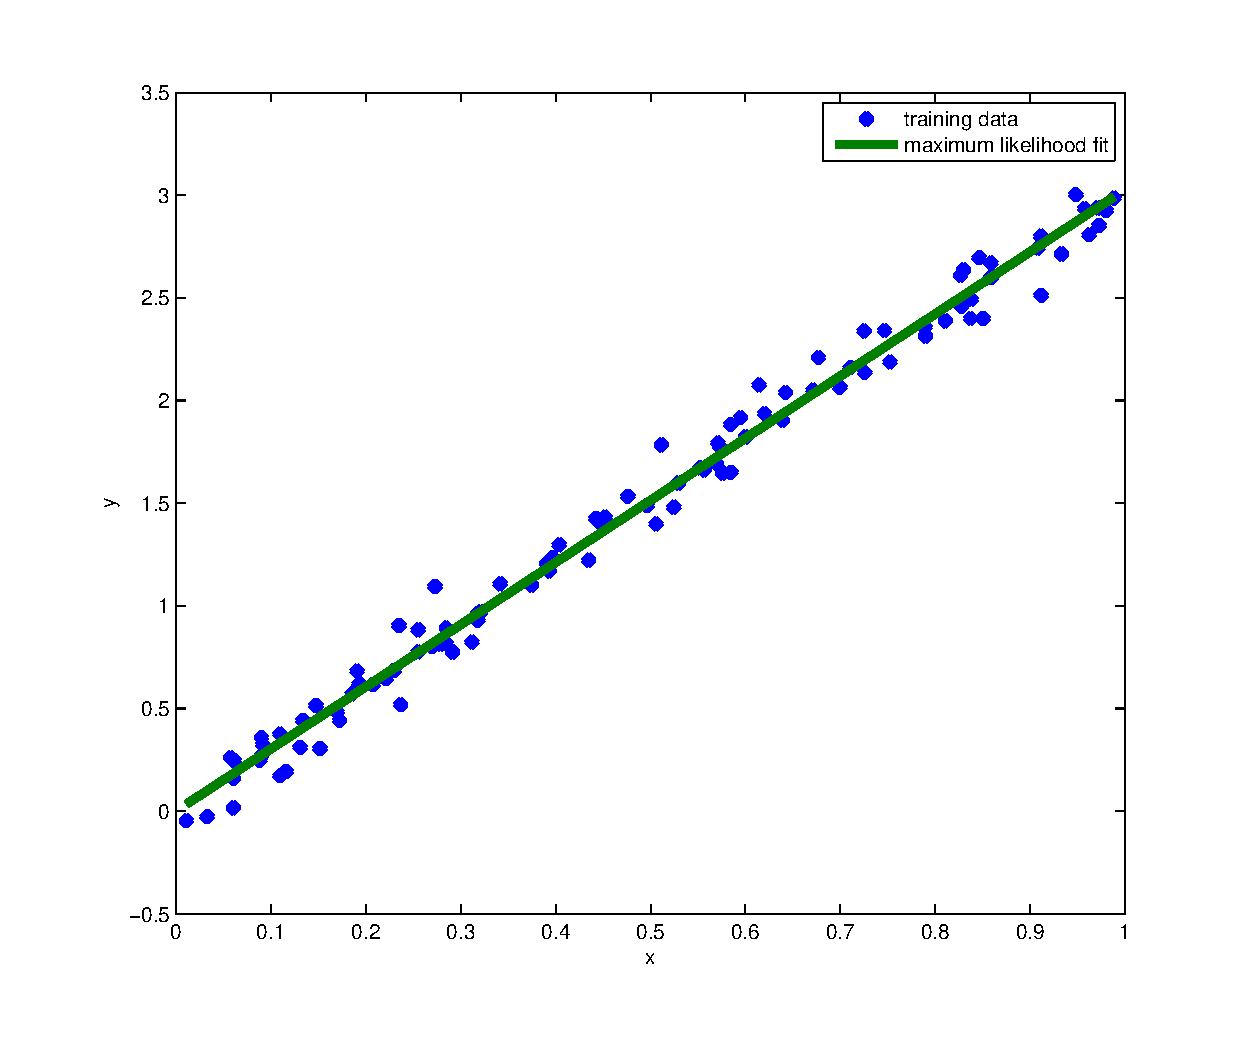
\includegraphics[width=6in,clip,keepaspectratio]{MLE.eps}\
			\caption{Estimation of $\theta$ with ML for linear regression}	
		\end{figure}
		
	\end{enumerate}
	
\section{Locally-weighted linear regression (20 points)}
	We need to fit $\theta$ to optimize cost function:	
	$$\Sigma_{i=1}^{m} w^{(i)} (\theta^T x^{(i)} - y^{(i)})^2$$
	
	Where $w$ are weights obtained by Gaussian kernel:
	$$w^{(i)} = exp(- \frac{||x^{(i)} - x||^2}{2\tau^2})$$
	
	In the example below training data is generated with sin function and some Gaussian noise. LWR gives the different fits with various $\tau$:
	
	\begin{figure}
		\centering
		\begin{subfigure}{.5\textwidth}
			\centering
			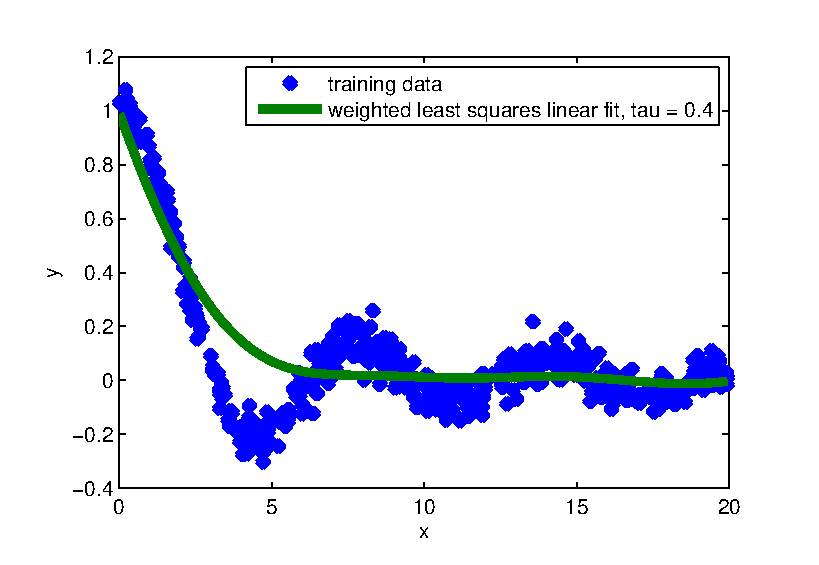
\includegraphics[width=.9\linewidth]{LWR-0-4.eps}
			\caption{$\tau = 0.4$: poor fit, oversimplified prediction}
			\label{fig:sub1}
		\end{subfigure}%
		\begin{subfigure}{.5\textwidth}
			\centering
			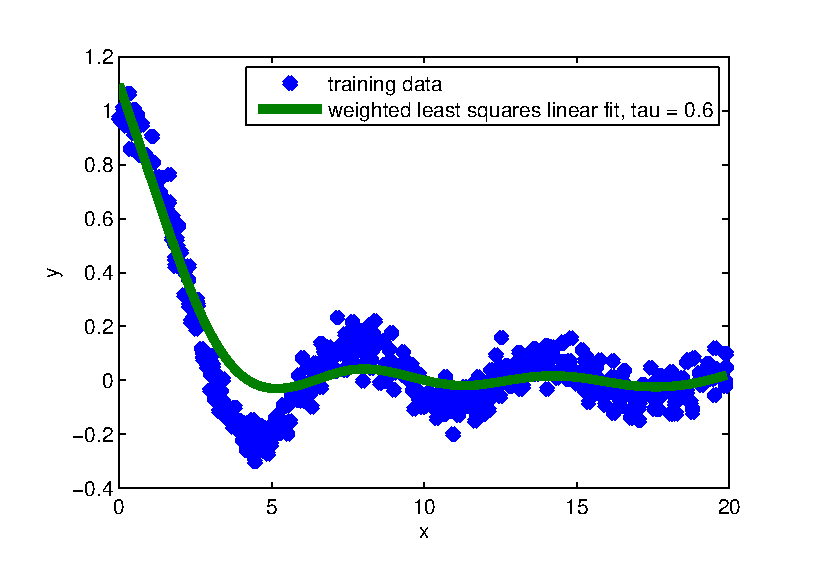
\includegraphics[width=.9\linewidth]{LWR-0-6.eps}
			\caption{$\tau = 0.6$: nice fit, reasonable prediction}
			\label{fig:sub2}
		\end{subfigure}
	\end{figure}	
	\begin{figure}
		\centering
		\begin{minipage}{.5\textwidth}
			\centering
			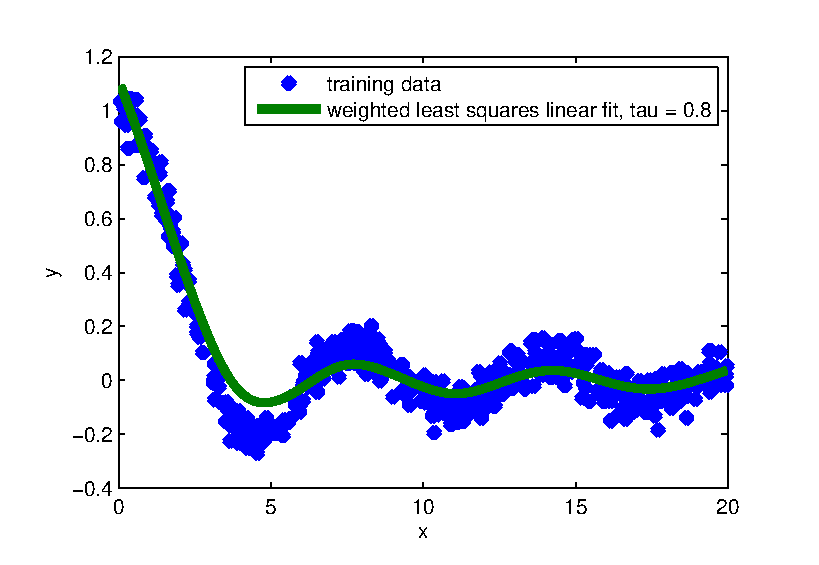
\includegraphics[width=.9\linewidth]{LWR-0-8.eps}
			\caption{$\tau = 0.8$: good fit, better prediction}
			\label{fig:sub1}
		\end{minipage}%
		\begin{minipage}{.5\textwidth}
			\centering
			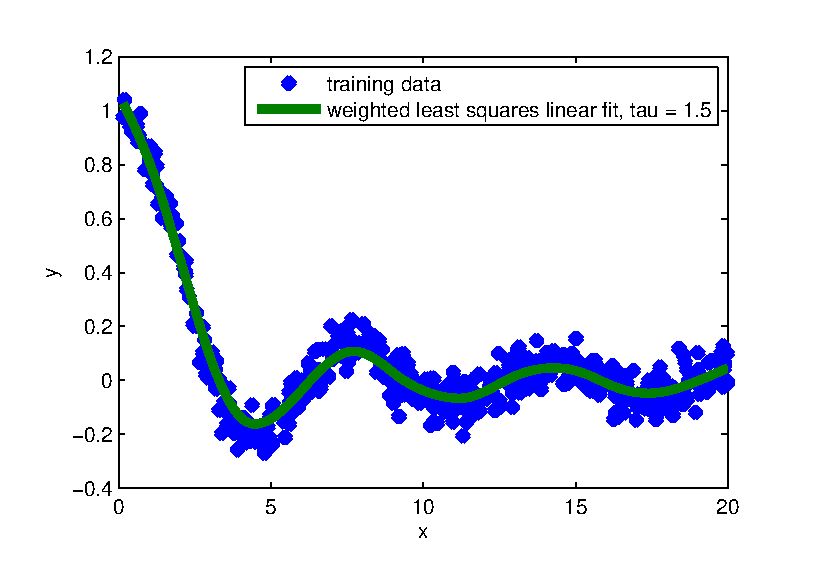
\includegraphics[width=.9\linewidth]{LWR-1-5.eps}
			\caption{$\tau = 1.5$: good fit, very accurate prediction}
			\label{fig:sub1}
		\end{minipage}
	\end{figure}	
	\begin{figure}
		\centering
		\begin{minipage}{.5\textwidth}
			\centering
			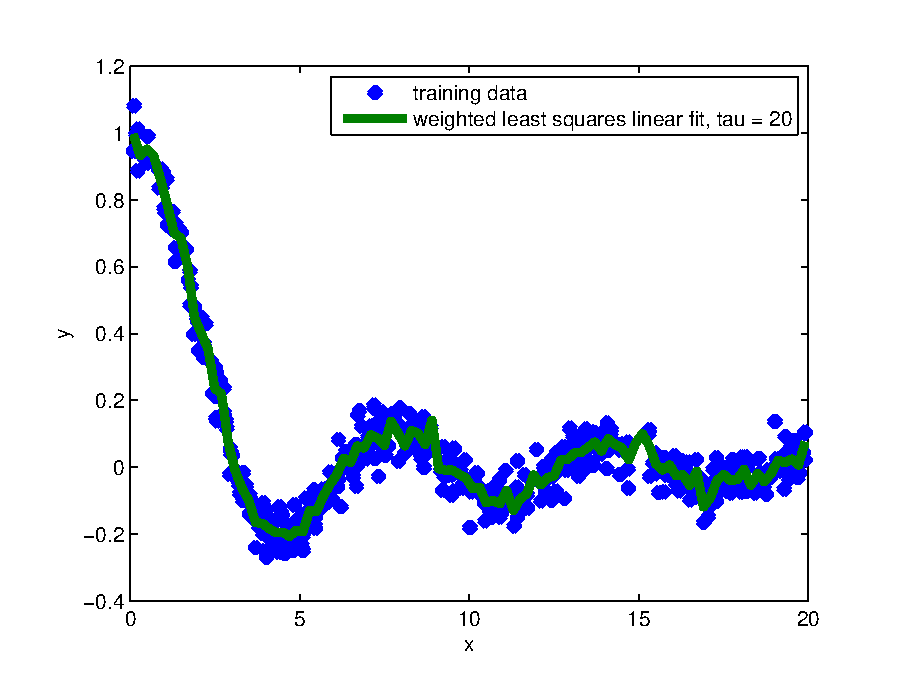
\includegraphics[width=.9\linewidth]{LWR-20.eps}
			\caption{$\tau = 20$: overfitting, useless prediction}
			\label{fig:sub1}
		\end{minipage}%
		\begin{minipage}{.5\textwidth}
			\centering
			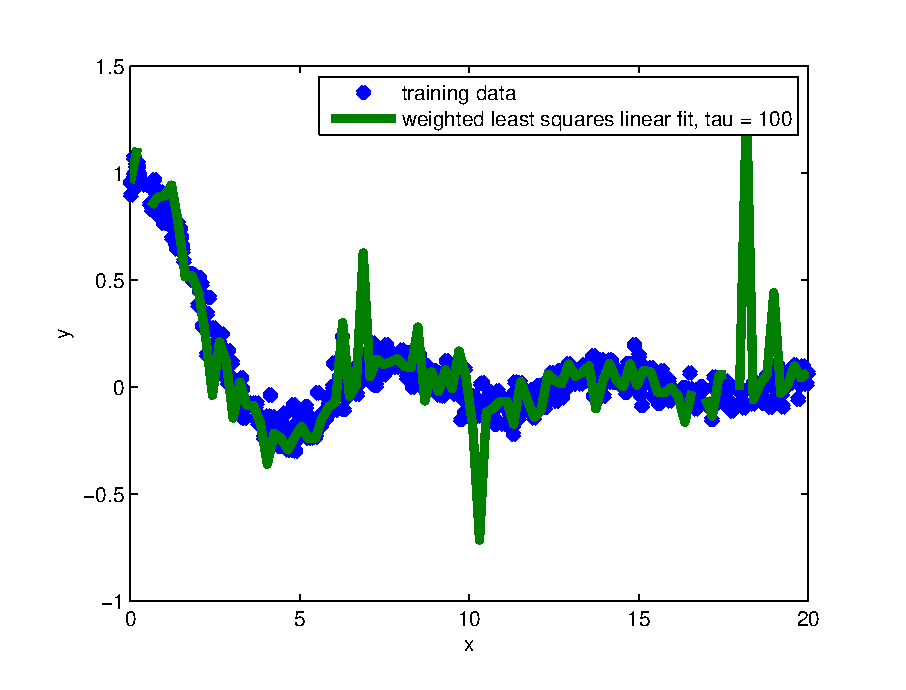
\includegraphics[width=.9\linewidth]{LWR-100.eps}
			\caption{$\tau = 100$: Heavy overfitting, wrong prediction}
			\label{fig:sub1}
		\end{minipage}
	\end{figure}


\section{Gradient descent, Newton's method, and logistic regression (30	points)}
	Although by implementing and using both algorithms we achieve convergence on learning for provided dataset, there are significant difference in approaches. 
	
	\subsection{Gradient Descent}
	First, let us take a look at Gradient Descent for Logistic Regression. The learning step is:
	$$\theta \leftarrow \theta + \alpha  \nabla_\theta l(\theta)$$
	First thing to notice: we have to choose learning rate $\alpha$ which is often undesirable for \textit{machine} learning. After first iteration we get different pictures depending on learning rate:
	\begin{figure}[h]
		\centering
		\begin{subfigure}{.5\textwidth}
			\centering
			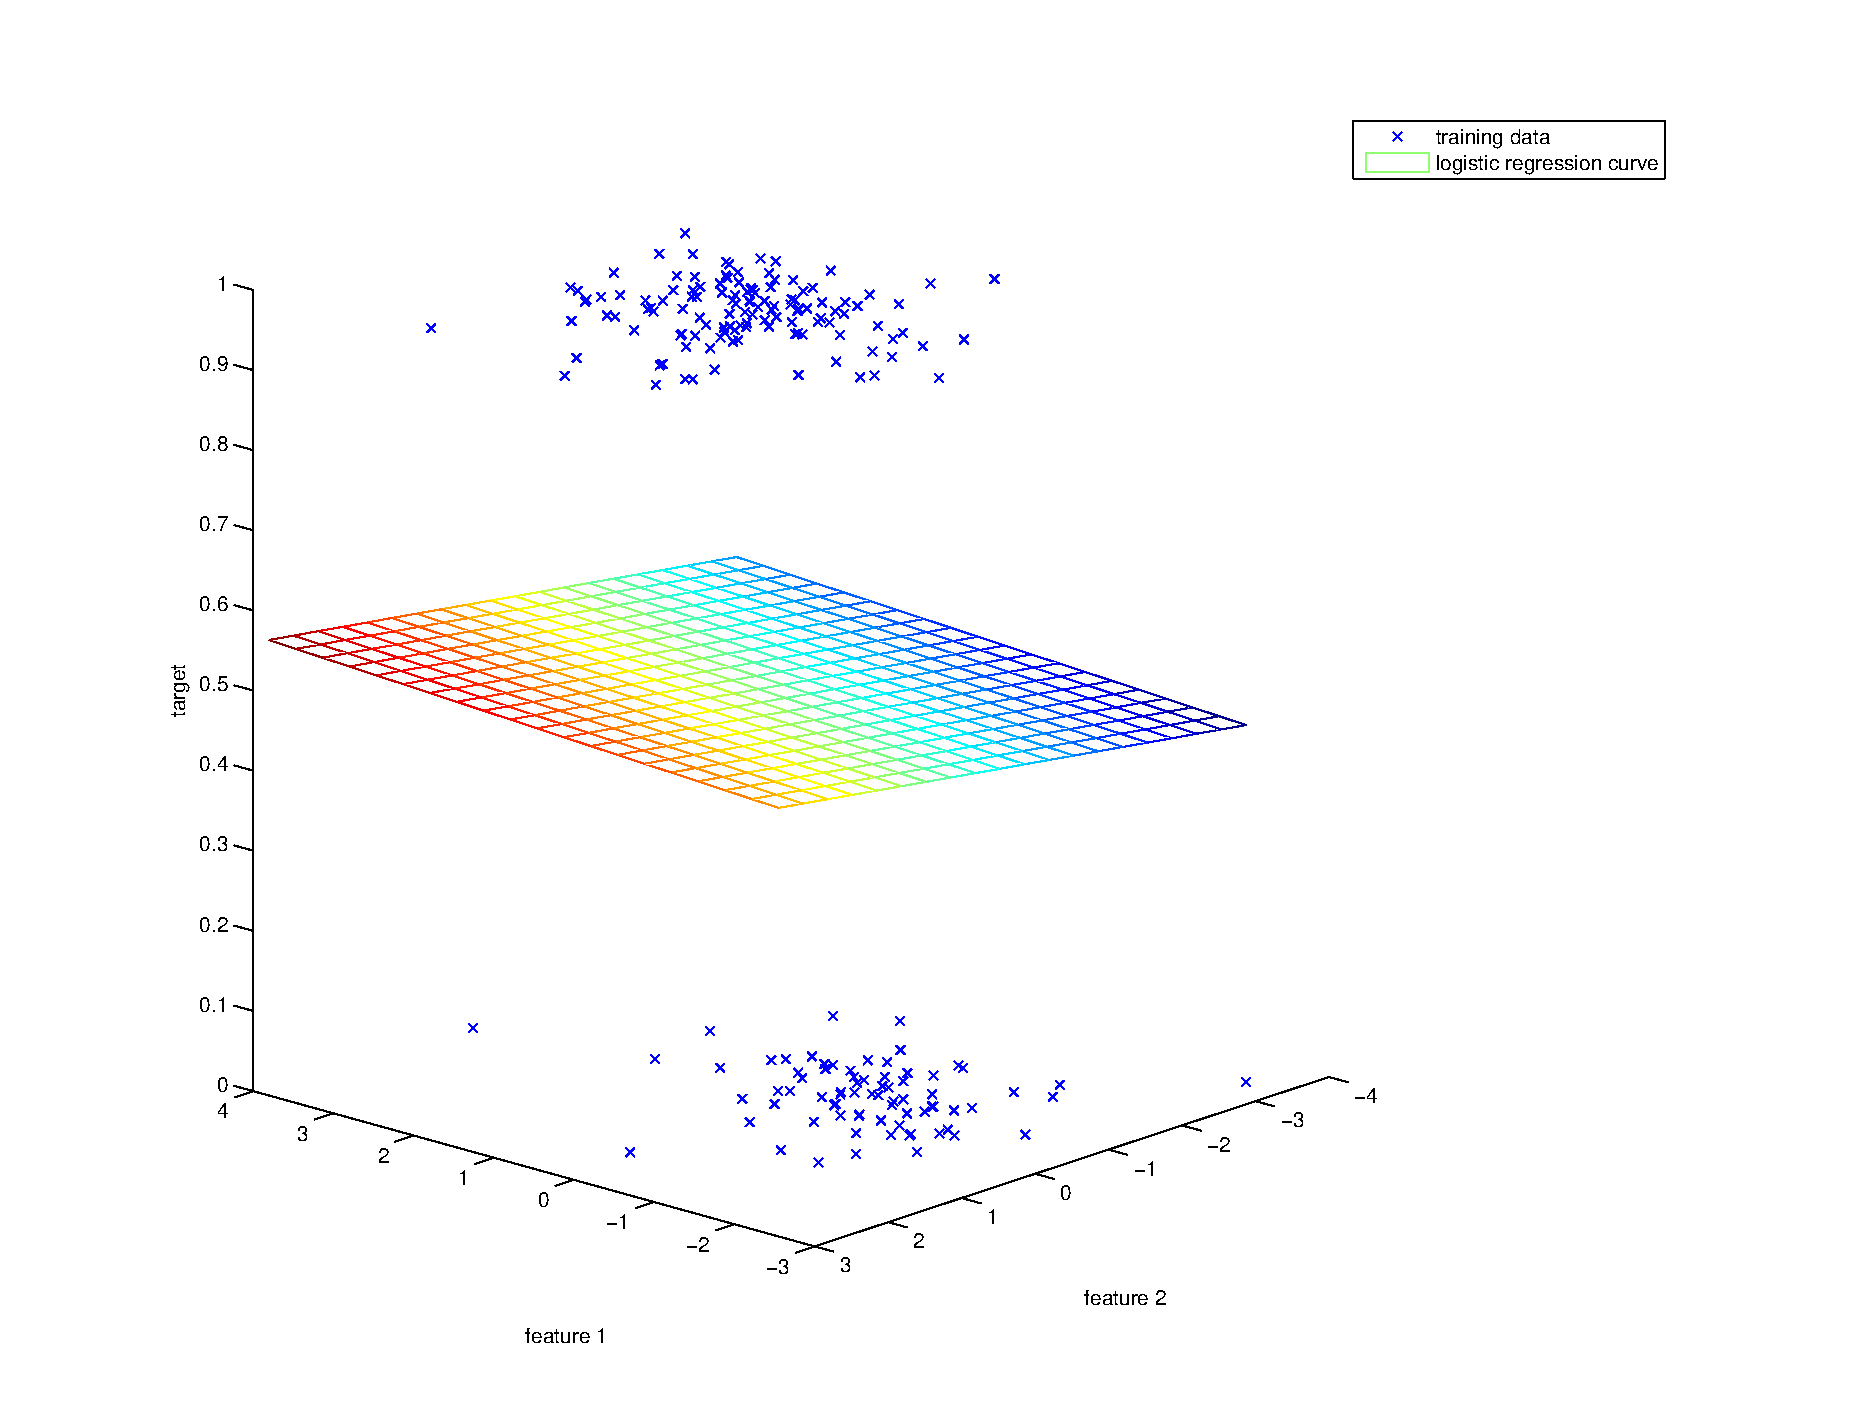
\includegraphics[width=.9\linewidth]{lr_provided_start_001.eps}
			\caption{$\alpha = 0.001$: Almost no learning}
			\label{fig:sub1}
		\end{subfigure}%
		\begin{subfigure}{.5\textwidth}
			\centering
			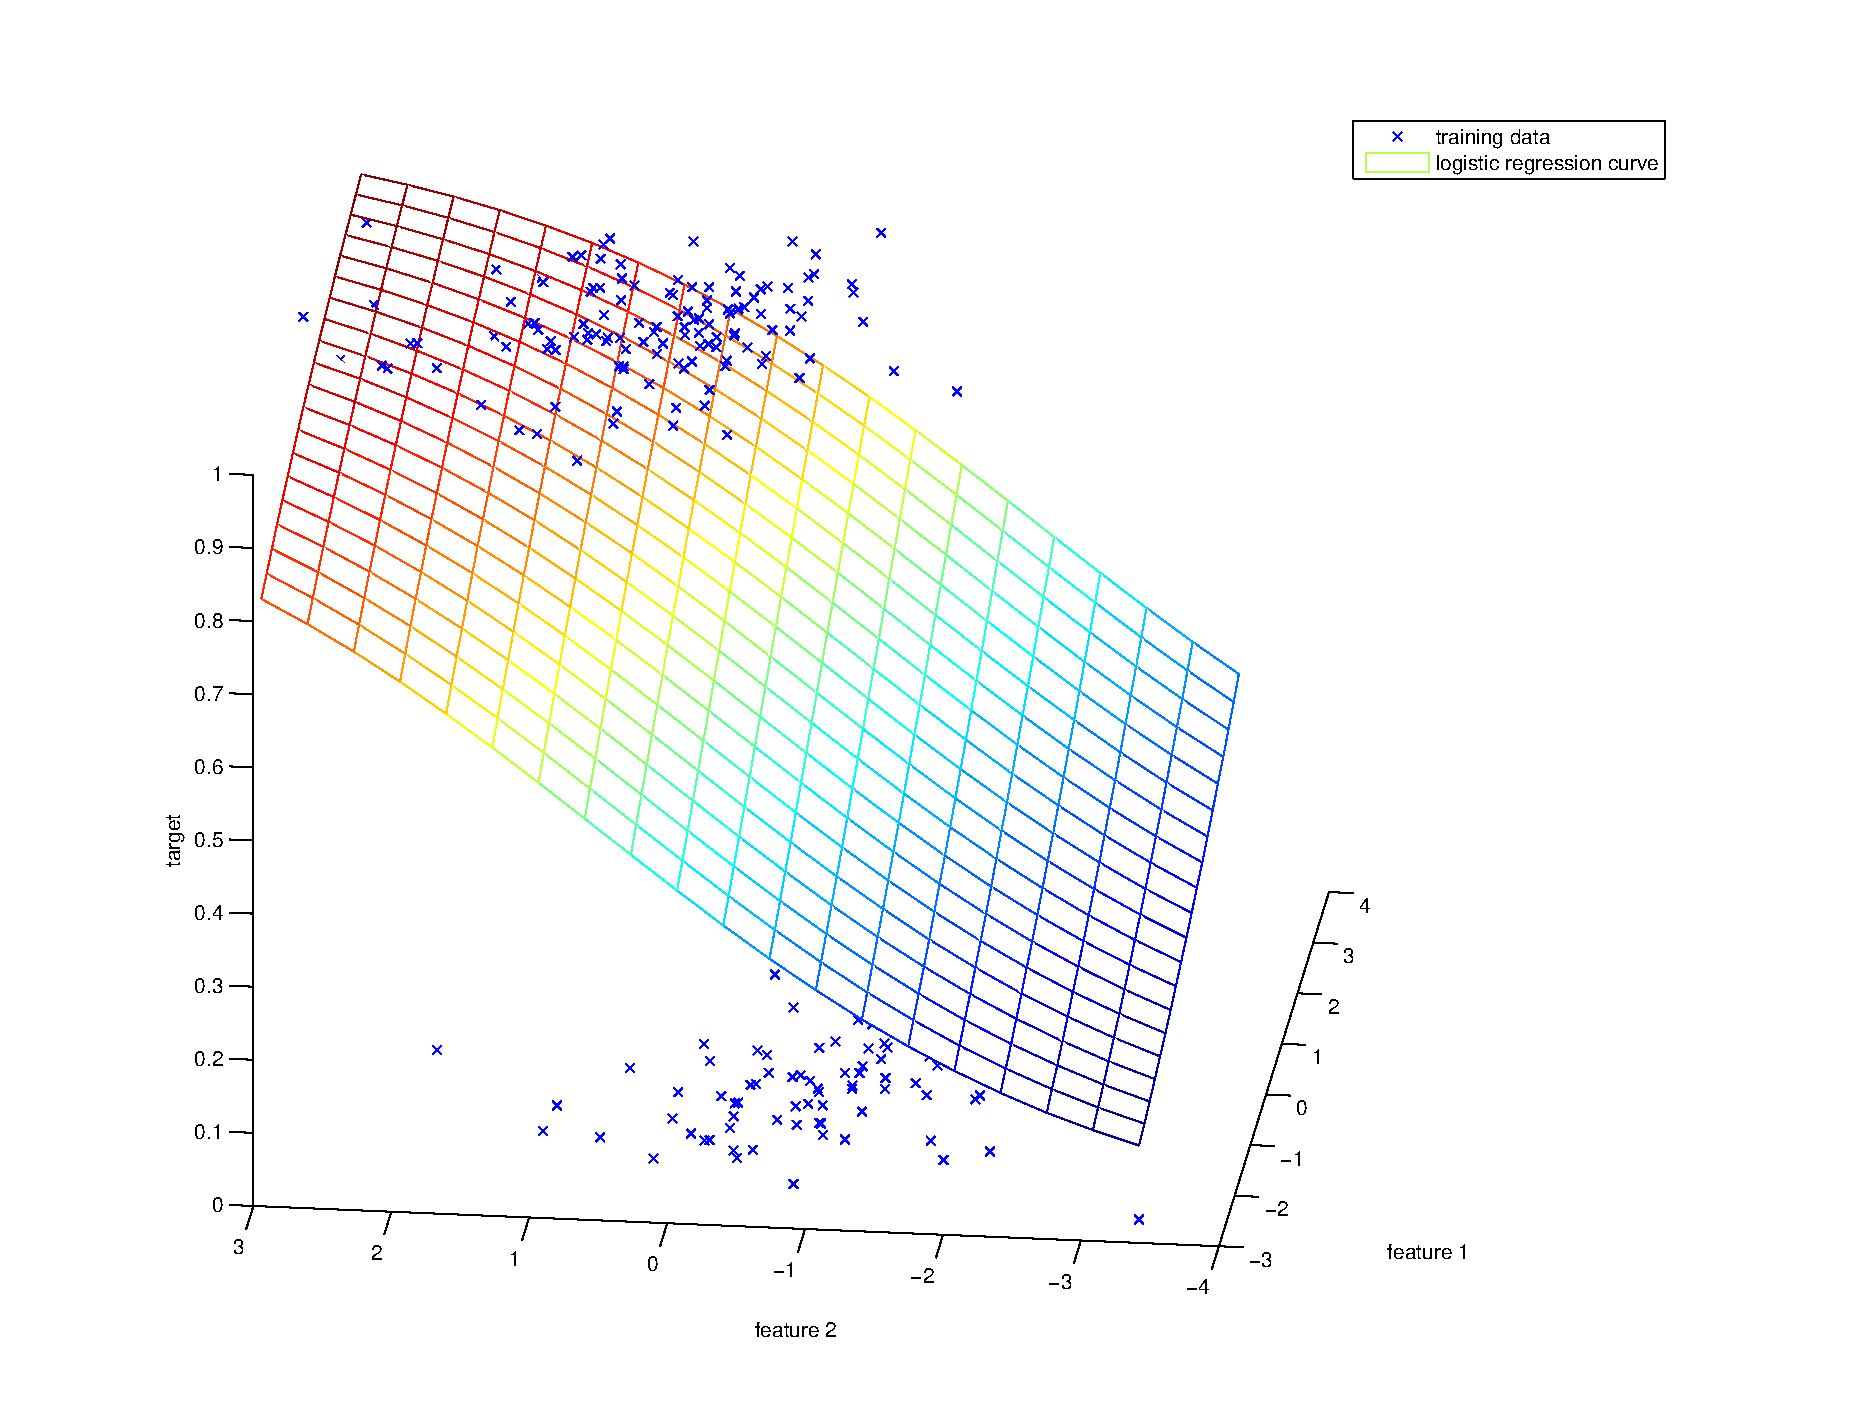
\includegraphics[width=.9\linewidth]{lr_provided_start_01.eps}
			\caption{$\alpha = 0.01$: reasonable improvement}
			\label{fig:sub2}
		\end{subfigure}
		\begin{subfigure}{.5\textwidth}
			\centering
			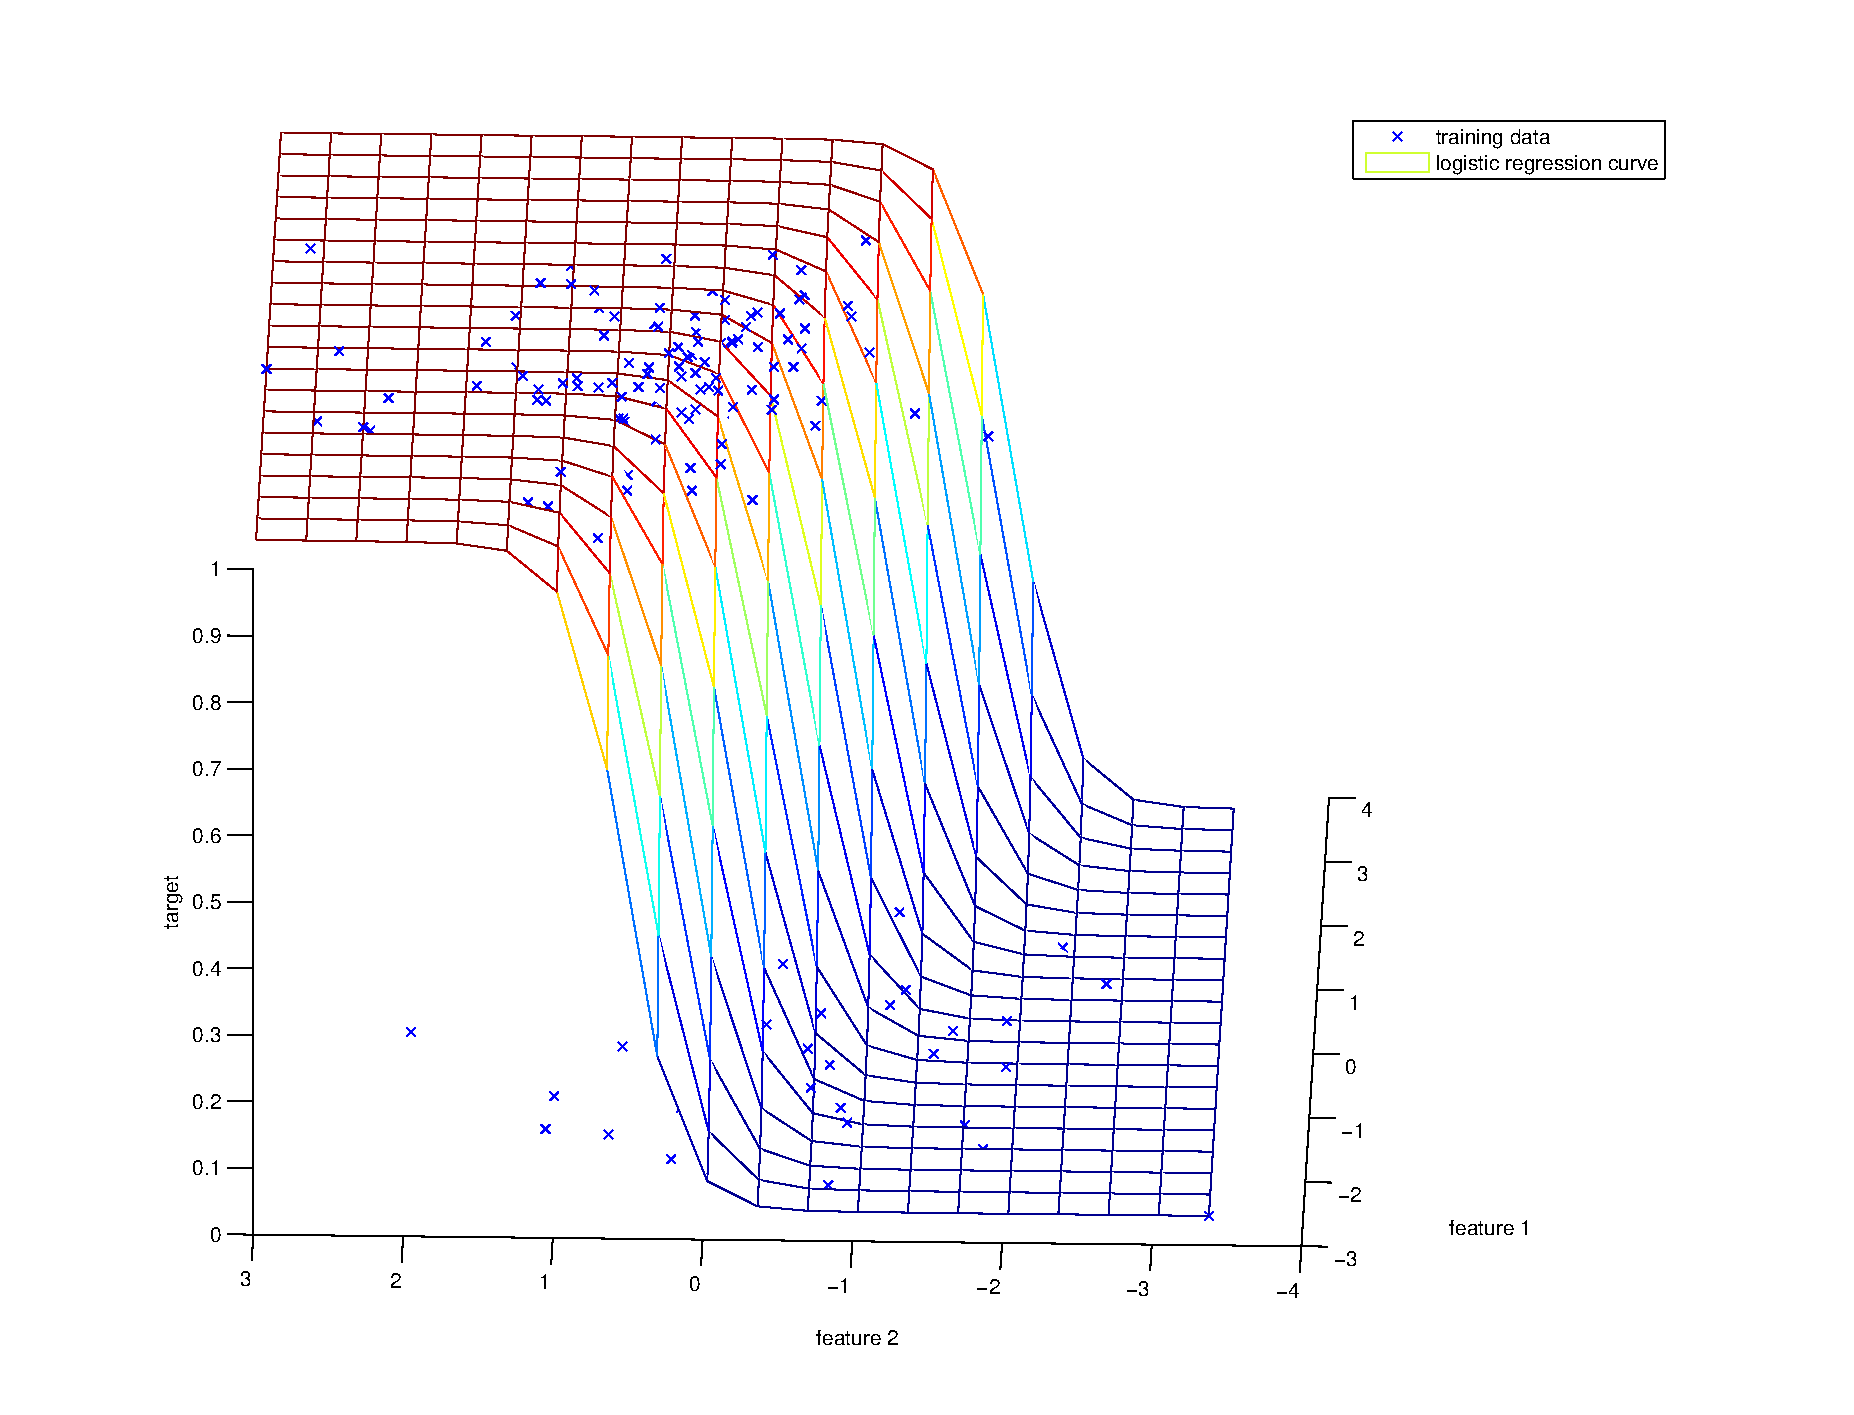
\includegraphics[width=.9\linewidth]{lr_provided_start_1.eps}
			\caption{$\alpha = 0.1$: seems like almost there}
			\label{fig:sub2}
		\end{subfigure}
	\end{figure}	
	\\Loigcally, higher the learning rate - faster the convergence (we will discuss the conditions later). However, that is not that simple.
	\begin{enumerate}
		\item Indeed, convergence happens faster for $\alpha = 0.01$ than $\alpha = 0.001$
		\item Too big learning rate, i.e. 0.1 leads to "jumping" behavior and not convergence at all. However this could be solved by decrementing learning rate by some percentage after each iteration.
	\end{enumerate}
	Conditions for convergence are:
	\begin{enumerate}
		\item accuracy = 1, where accuracy is number correct guesses divided by number of examples
		\item norm(H) $<$ 1e-10 
		\item norm(grad) $<$ 1e-10
	\end{enumerate}
	While dataset provided has overlapping values we never reach the accuracy condition. However, we can add another condition about accuracy not changing much (or at all). For instance, for given dataset, maximum accuracy is 0.835. Method described above converges to this value over 9 iterations (with $\alpha = 0.01$).
	
	\subsection{Newton's method}
	For Newton's method, the learning step is:
	$$\theta \leftarrow \theta - H'  \nabla_\theta l(\theta)$$
	where $H$ is a Hessian matrix, which basically contains second partial derivatives. 
	
	Intuitively, Newton's method converges faster. On provided dataset we have this picture after two iterations:
	\begin{figure}[h]
		\centering
		\begin{subfigure}{.5\textwidth}
			\centering
			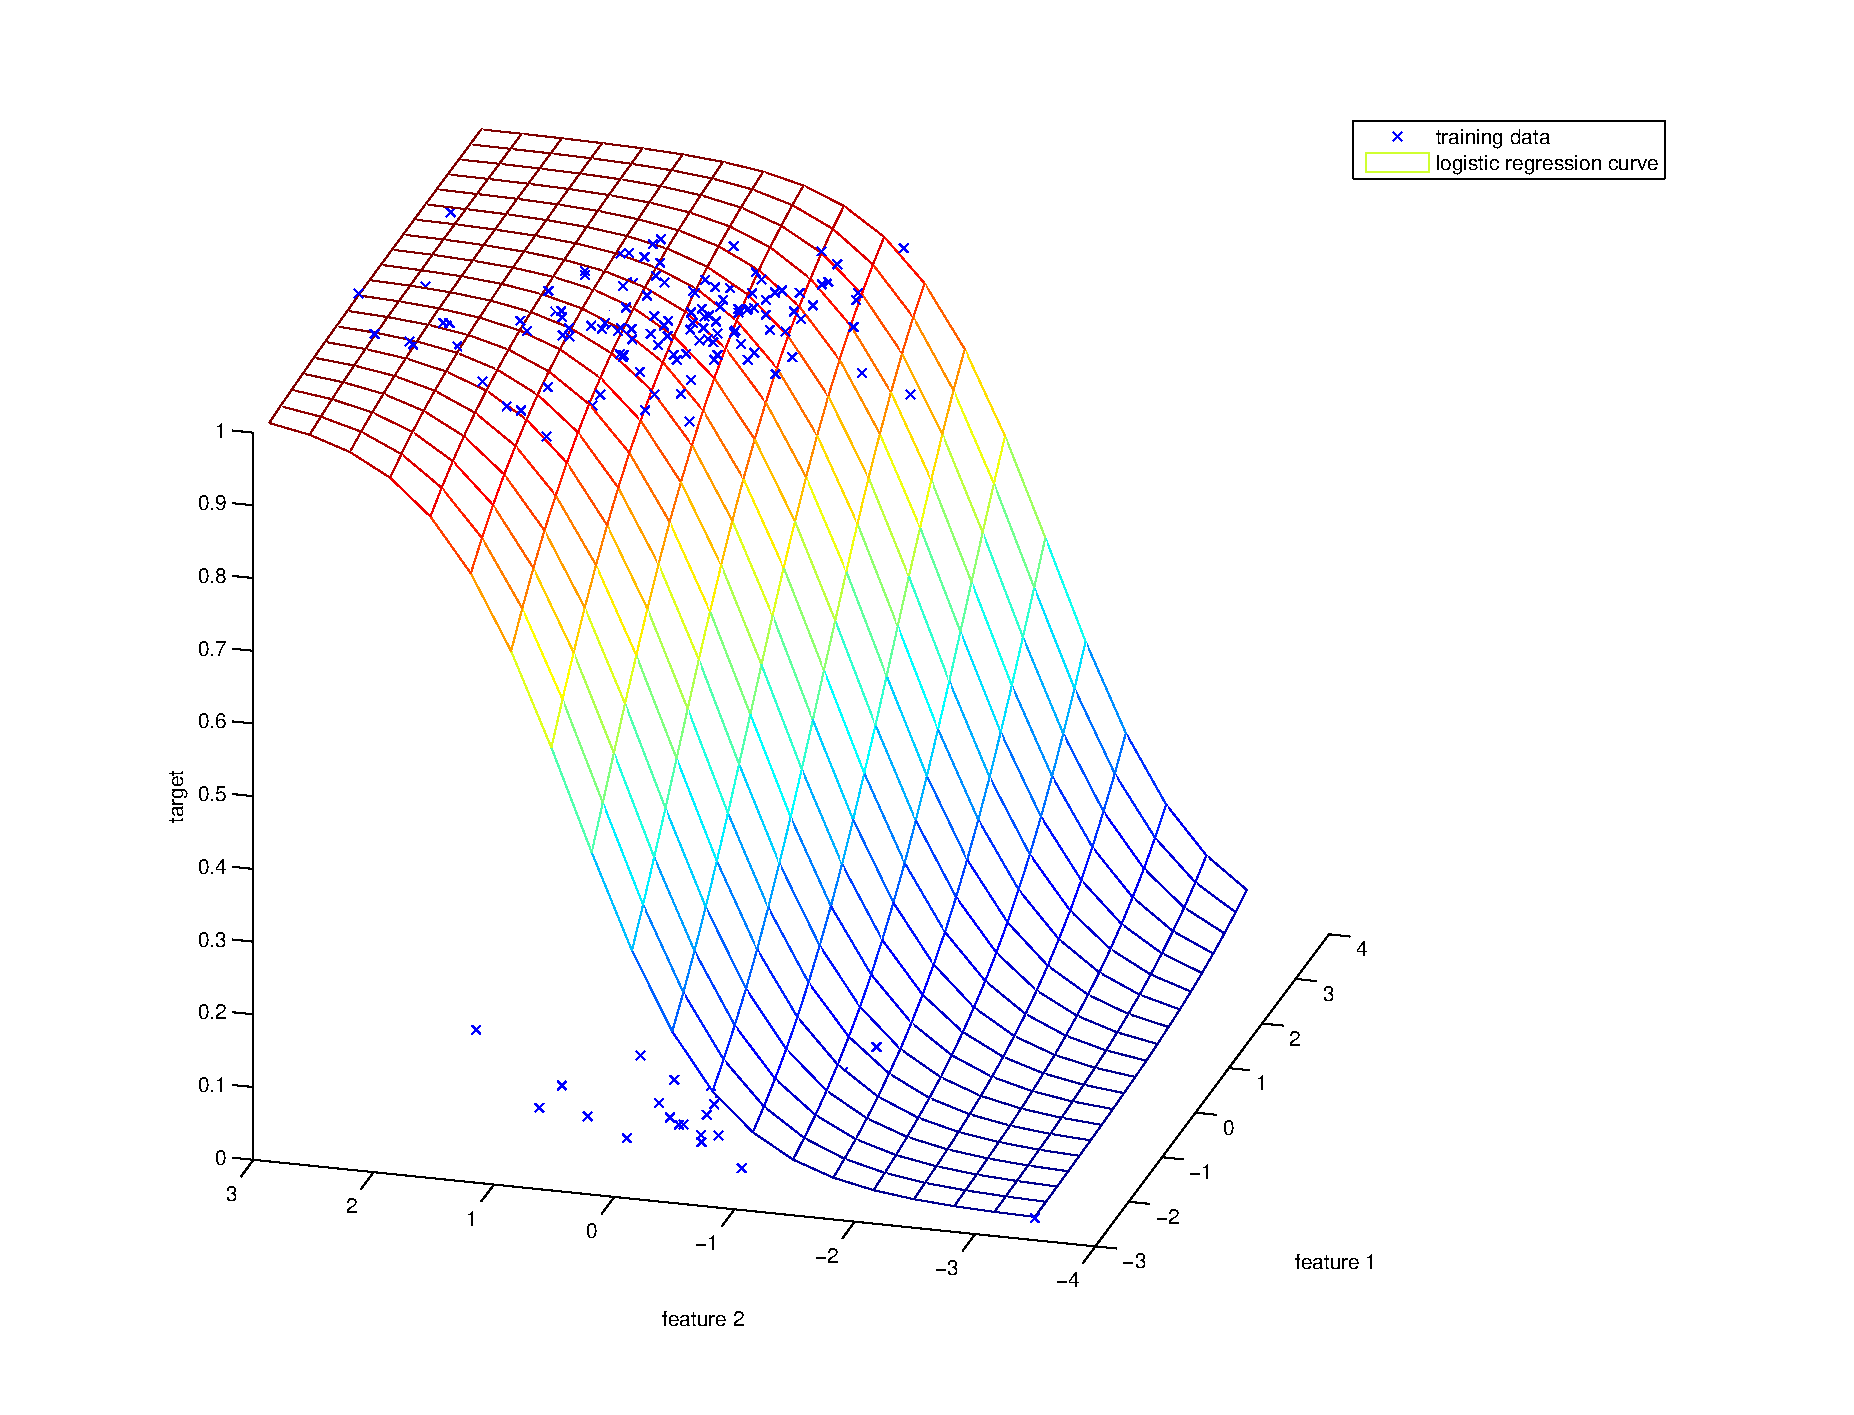
\includegraphics[width=.9\linewidth]{lr_provided_start_newton_2.eps}
			\caption{Newton's method after 2 iteration: accuracy = 0.830}
			\label{fig:sub1}
		\end{subfigure}%
	\end{figure}	
	That is almost maximum accuracy that possible on the dataset. Method converges after 7 iterations because of norm(H) condition. 
	
	\subsection{Convenient dataset}
	For testing purposes we create convenient dataset with clear division:
	\pagebreak
	\begin{lstlisting}[frame=single,basicstyle=\ttfamily]
testx1 = rand(m, 1) * 20 - 10; %generate some rand x
testx2 = rand(m, 1) * 50 - 25;
testy = zeros(m, 1);
%make separation clear
testx1((testx2 + testx1) < 10 & (testx2 + testx1) > 7) = 0; 
testx2((testx2 + testx1) < 10 & (testx2 + testx1) > 7) = 0;
testy((testx2 + testx1) > 10) = 1; % arbitrary classification   
testx = [testx1, testx2]; %combine features
	\end{lstlisting}
	
	Gradient Descent doesn't converge after 100 iterations:
	\begin{figure}[h]
		\centering
		\begin{subfigure}{.5\textwidth}
			\centering
			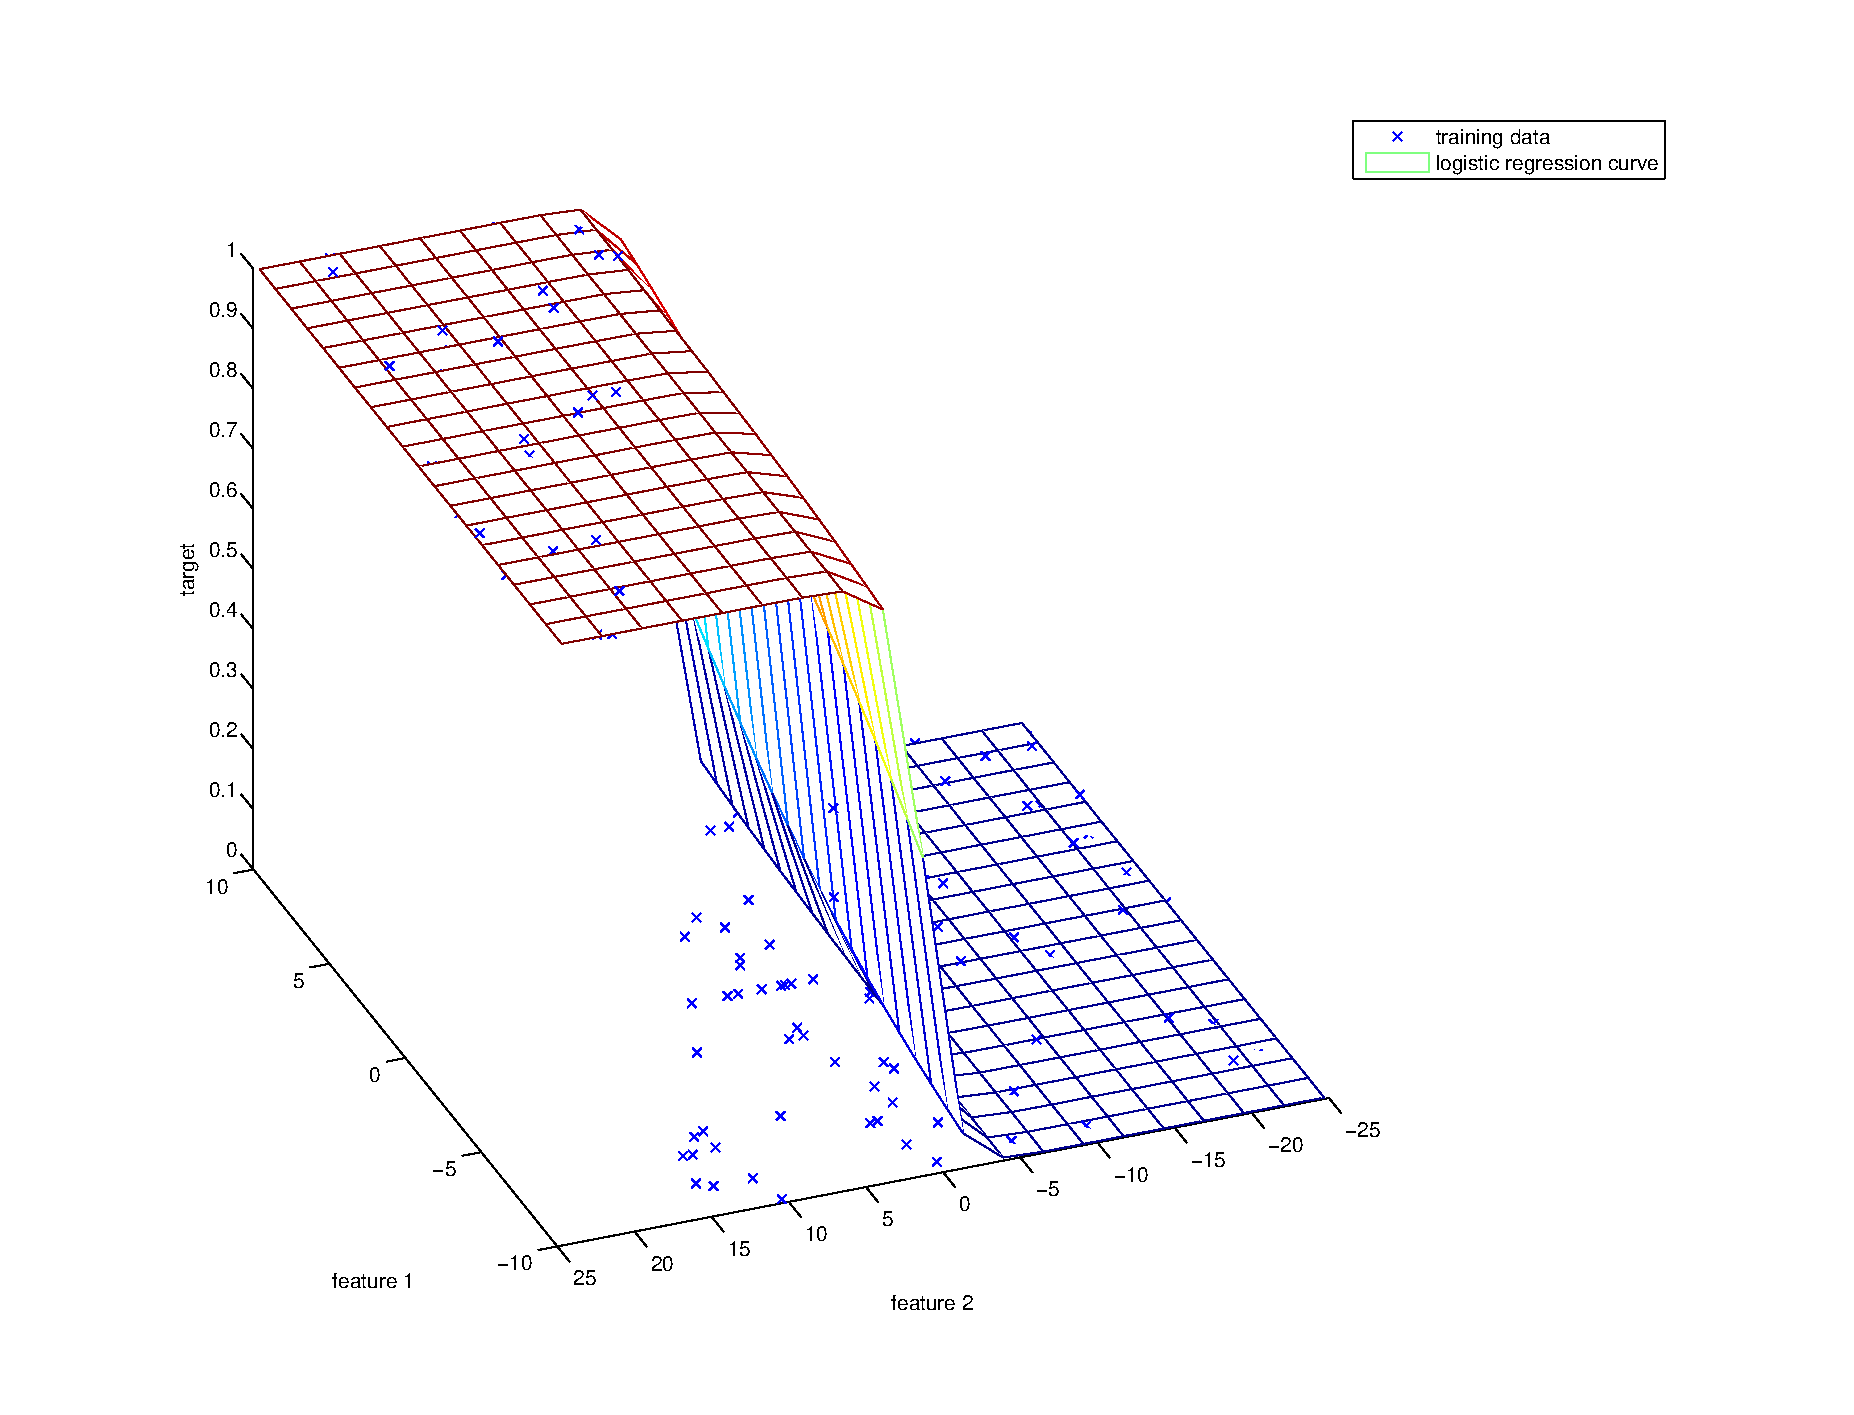
\includegraphics[width=.9\linewidth]{testdataset_gd_start.eps}
			\caption{Gradient Descent after 1 step}
			\label{fig:sub1}
		\end{subfigure}%
		\begin{subfigure}{.5\textwidth}
			\centering
			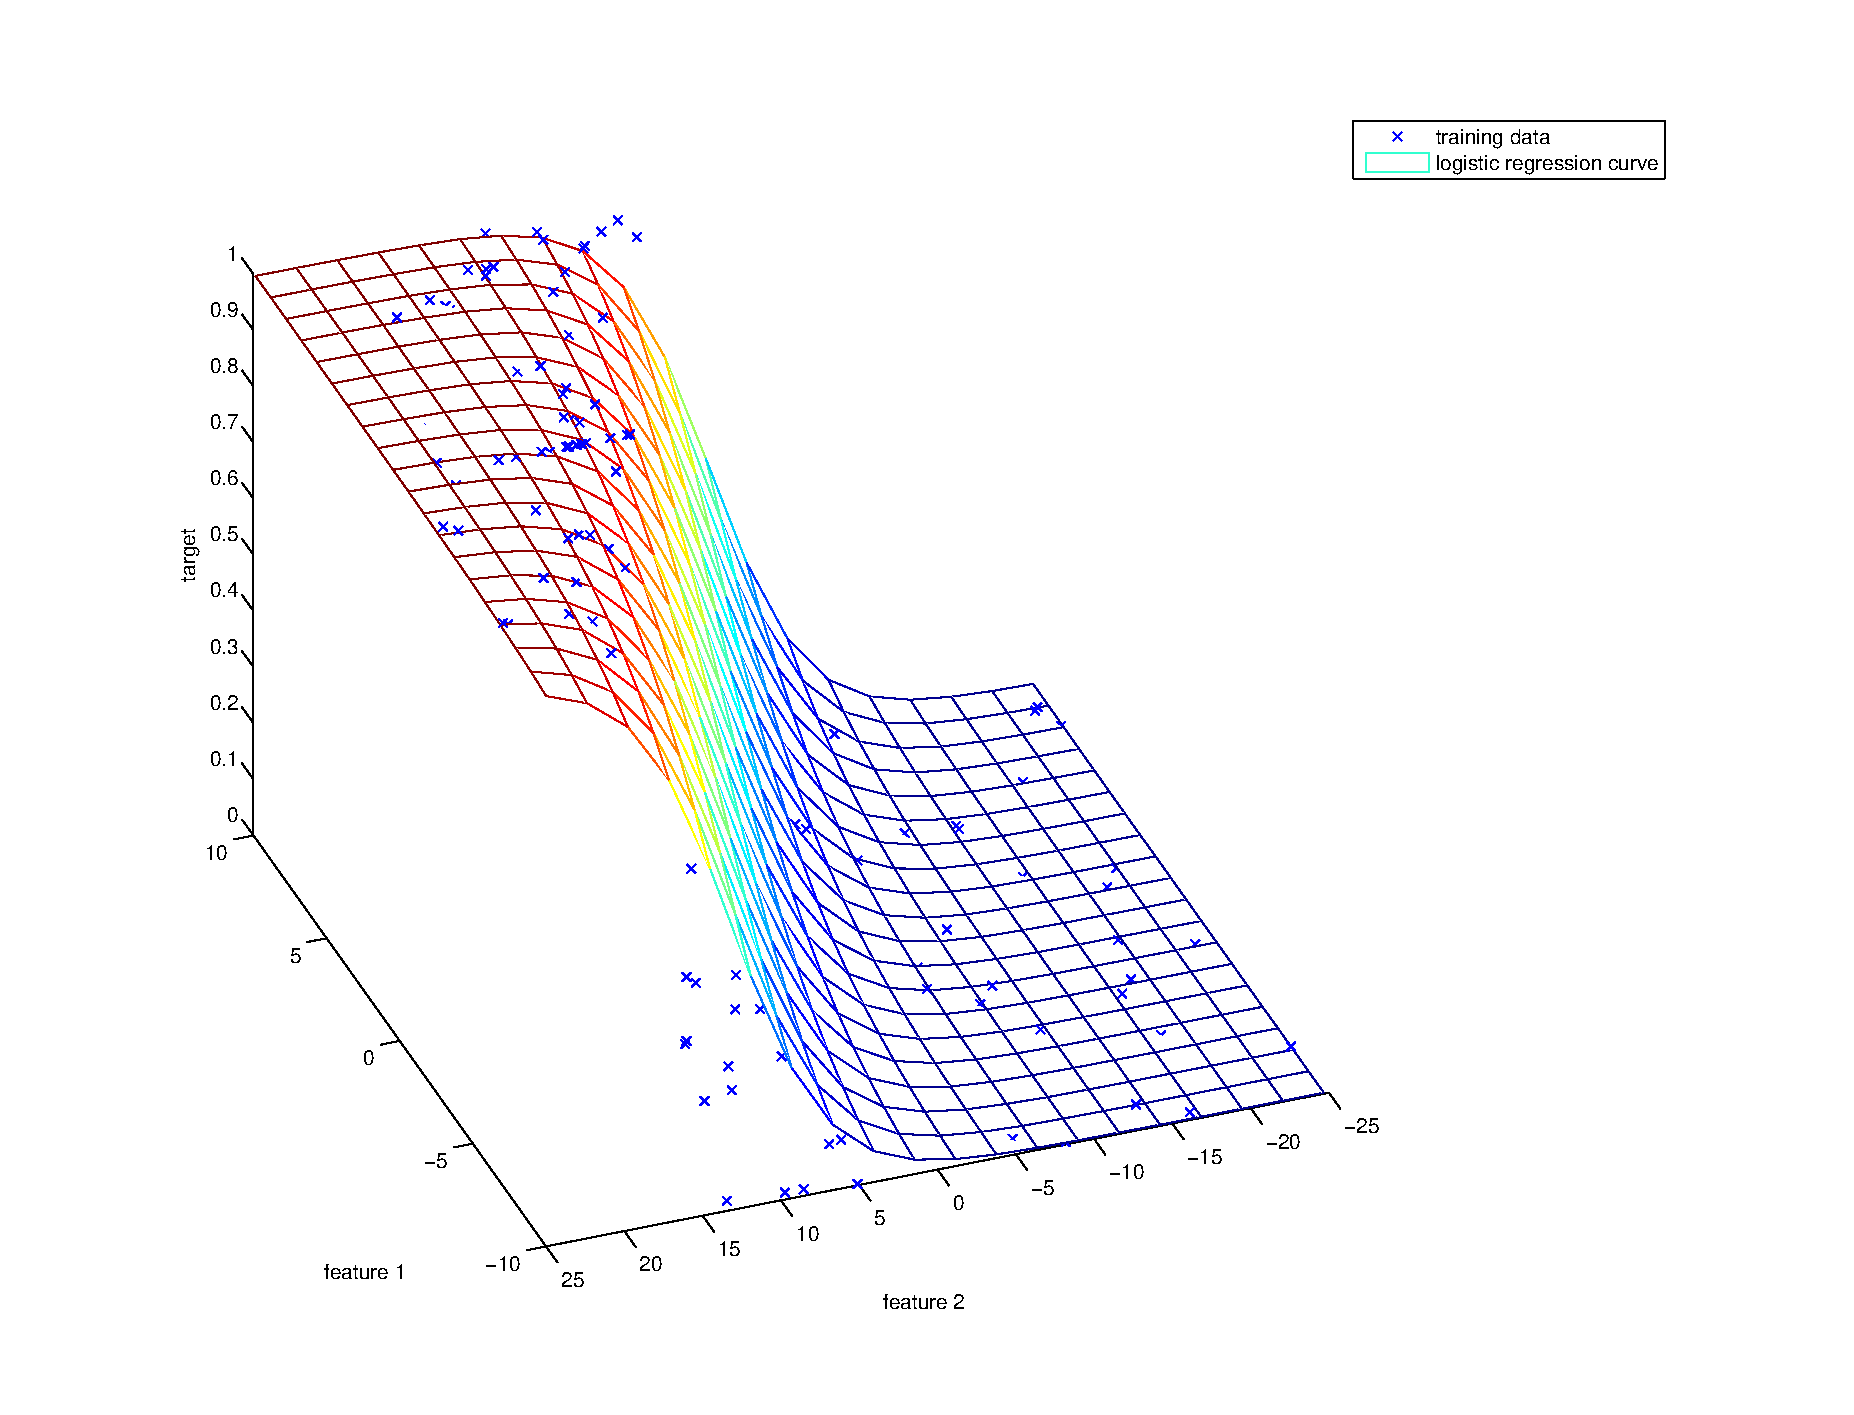
\includegraphics[width=.9\linewidth]{testdataset_gd_end.eps}
			\caption{Gradient Descent after 100 steps. Accuracy = 0.93}
			\label{fig:sub2}
		\end{subfigure}
	\end{figure}
	
	Newton's method converges after 4 iterations with perfect accuracy:
	\begin{figure}[h]
		\centering
		\begin{subfigure}{.5\textwidth}
			\centering
			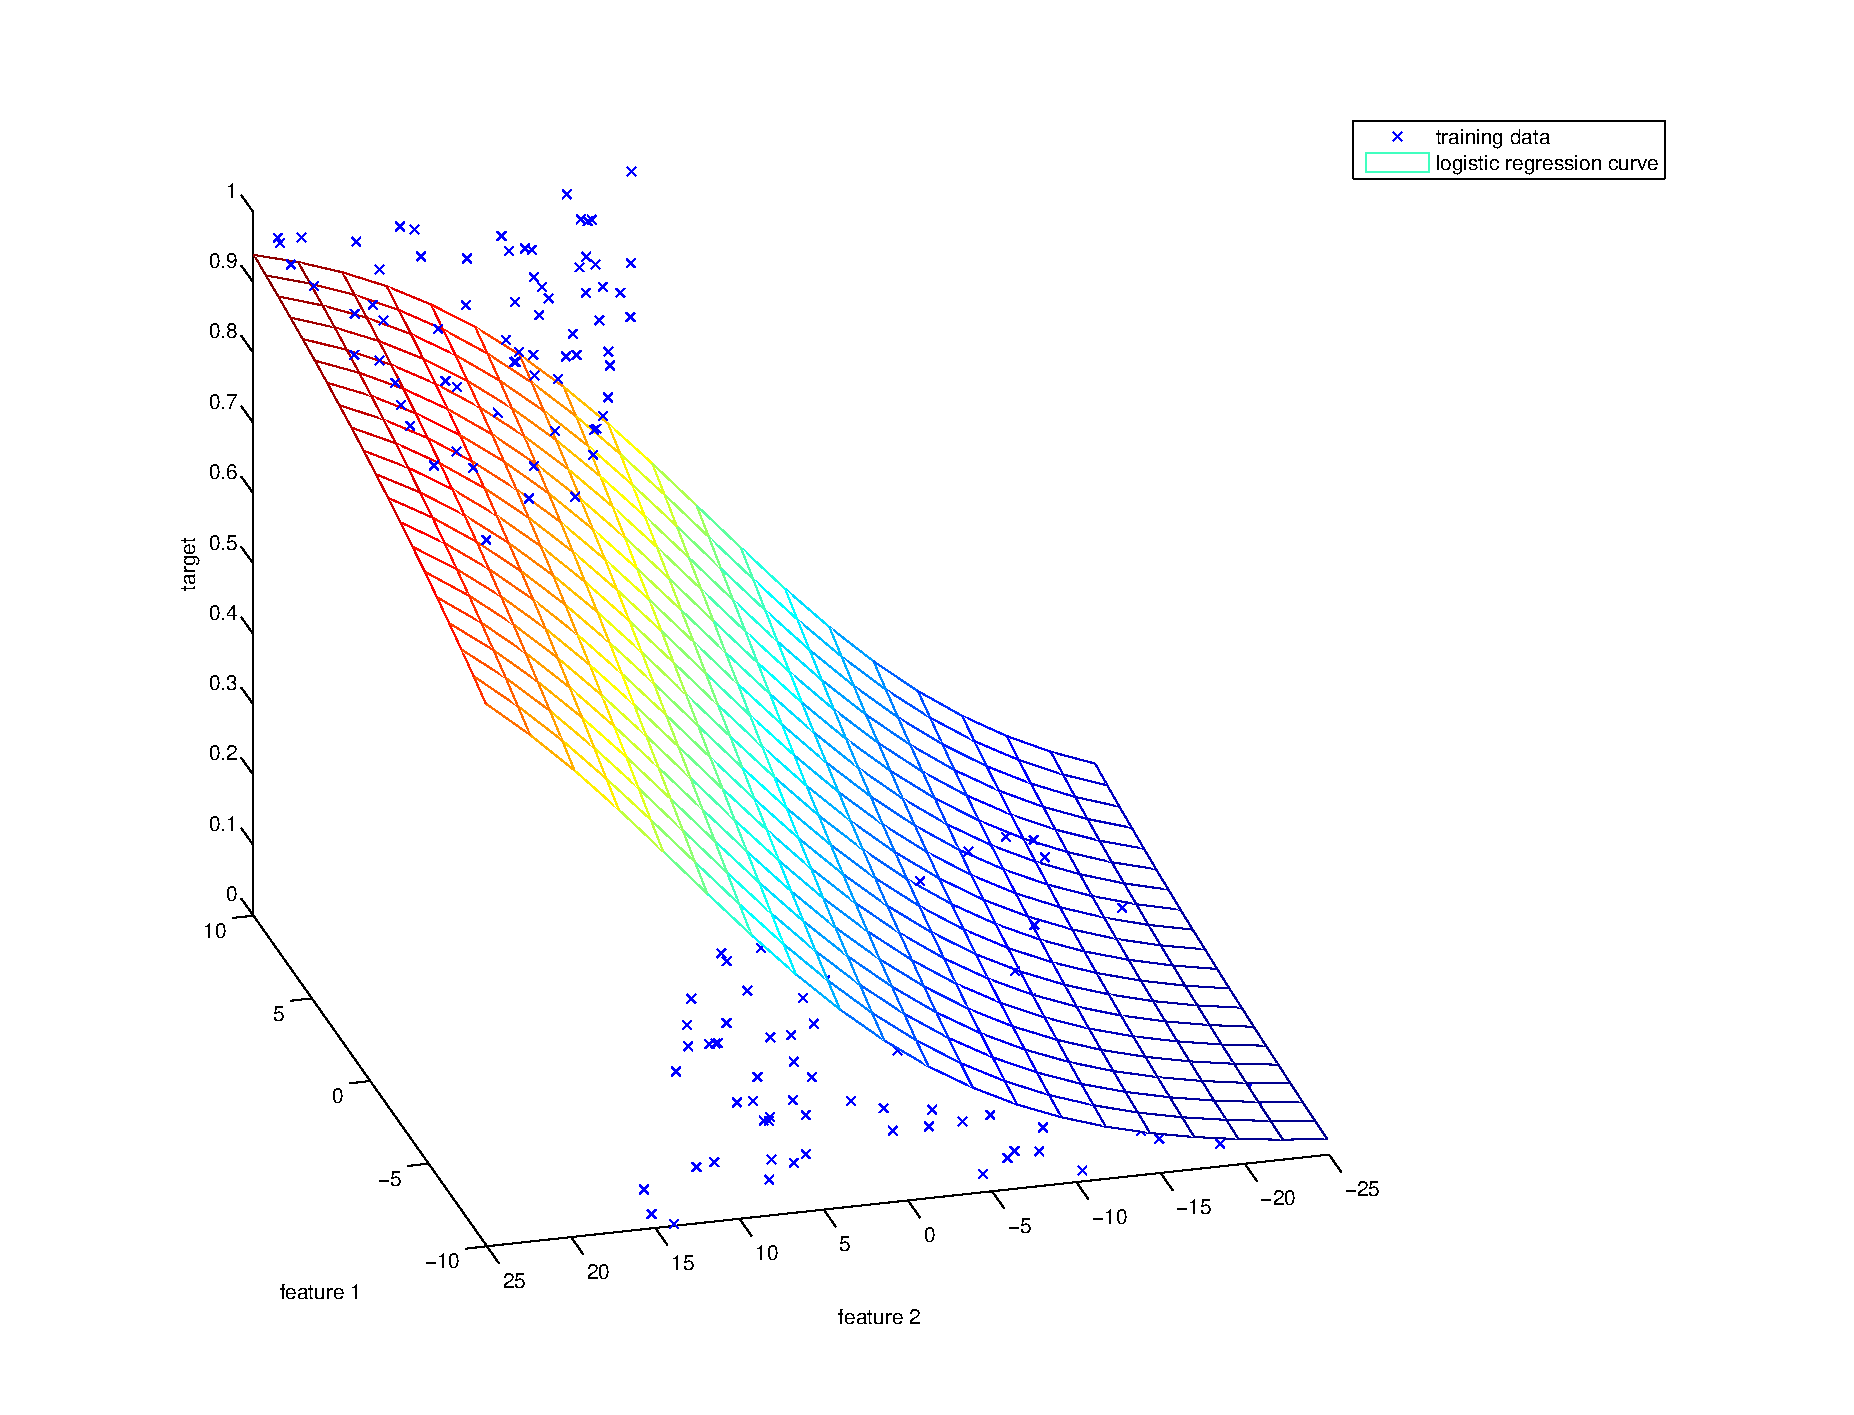
\includegraphics[width=.9\linewidth]{testdataset_newton_start.eps}
			\caption{Newton's method after 1 step}
			\label{fig:sub1}
		\end{subfigure}%
		\begin{subfigure}{.5\textwidth}
			\centering
			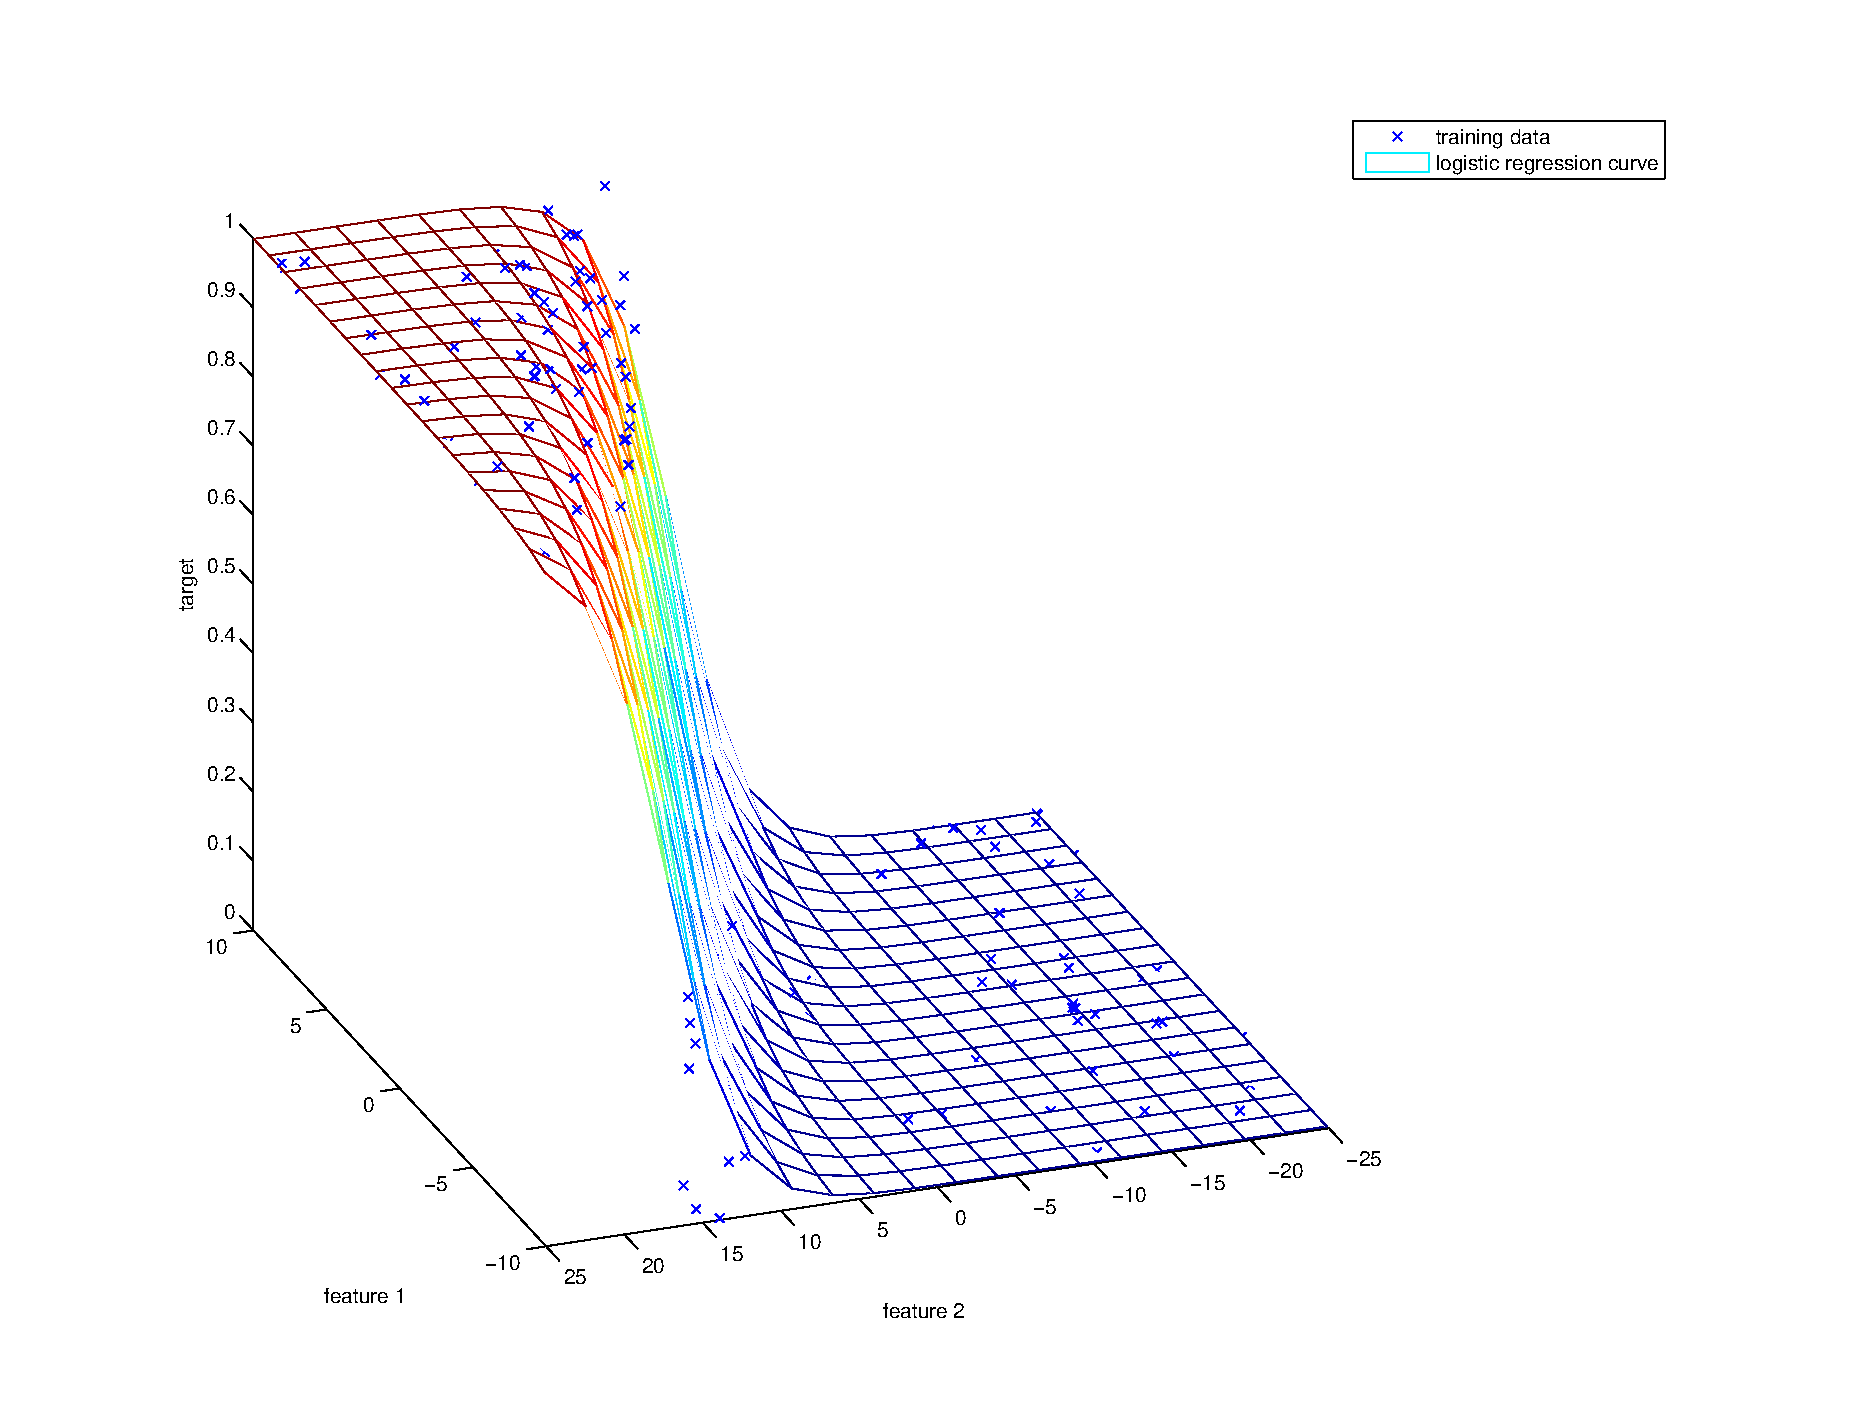
\includegraphics[width=.9\linewidth]{testdataset_newton_end.eps}
			\caption{Converges after 4 iterations with accuracy = 1}
			\label{fig:sub2}
		\end{subfigure}
	\end{figure}

	\pagebreak
	\subsection{Theta behavior without accuracy condition}
	If we eliminate stopping condition of accuracy, both methods tend to amplify $\theta$ thus narrowing the Sigmoid's "bump". 
	\begin{figure}[h]
		\centering
		\begin{subfigure}{.5\textwidth}
			\centering
			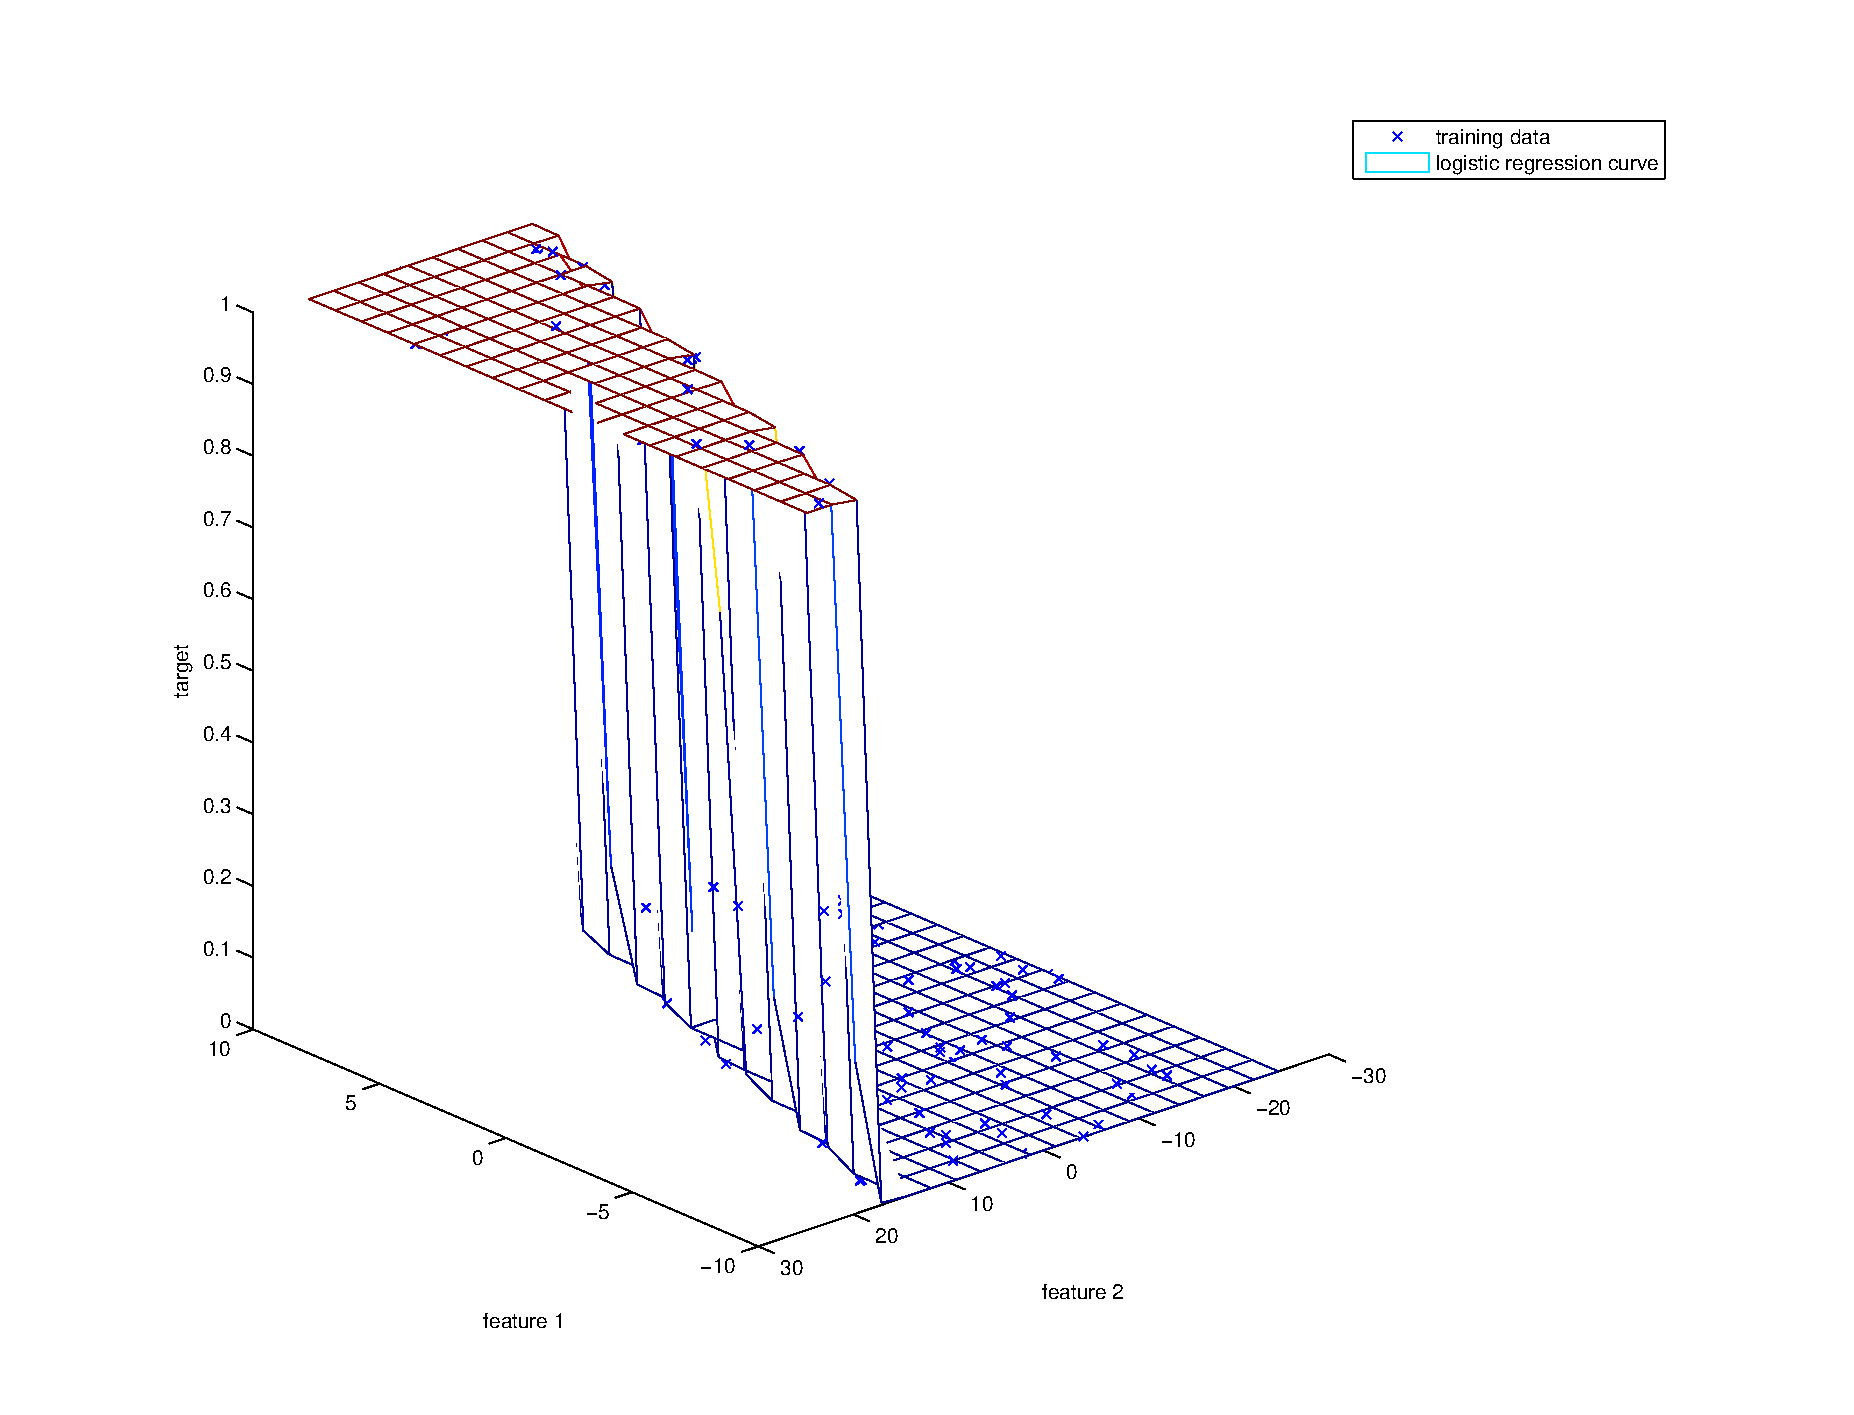
\includegraphics[width=.9\linewidth]{testdataset_no_accuracy_condition.eps}
			\caption{Newton's method after 13 iteration without accuracy stopping condition}
			\label{fig:sub1}
		\end{subfigure}%
	\end{figure} 
	\\That behavior continues until norma of gradient or Hessian matrix is too small. For test dataset we receive $\theta$ = (-133.0180 15.6132 15.7568) instead of appropriate  (-4.9162	0.5683	0.6271).
	
\section{Extra credit 1: deriving logistic regression (+5 points)}
	Show the derivations for the gradient and the Hessian of the log-likelihood for logistic regression.\\
	We'll use the following rules of derivative:
	\begin{enumerate}
		\item $log'(x) = \frac{1}{x}$
		\item $(f(g(x)))' = f'(g(x)) * g'(x)$
		\item $f'(x) = f(x)(1-f(x))$
		\item $\nabla$ is a set of partial derivatives
	\end{enumerate}
	So if:
	\begin{align*}
	\ell(\theta) &= logL(\theta)\\
	&= \sum_{i=1}^{m} y^{(1)} \log h_{\theta}(x^{(i)}) + (1-y^{(1)}) \log (1 - h_{\theta}(x^{(i)})) 
	\end{align*}
	Where:
	$$h_{\theta}(x) = g(\theta^T x)$$
	
	Then partial derivative for one example (x, y) with respect of $\theta_j$:
	$$
	\patheta \elll = (y \frac{1}{g(\theta^T x)} - (1-y)\frac{1}{g(1-\theta^T x)}) \patheta g(\thetax) $$
	
	By (2) and (3): 
	\begin{align*} \patheta g(\thetax) &= g(\thetax)(1 - g(\thetax)) \patheta \thetax\\
	&= g(\thetax)(1 - g(\thetax)) x_j 
	\end{align*}
	
	Plug it back and simplify:
	\begin{align*}
	\patheta \elll &= (y(1-g(\thetax)) - (1-y)g(\thetax))x_j\\
	&= (y-g(\thetax))x_j 
	\end{align*}
	
	Then the gradient for several features for one example would be a vector with values for various j:
	$$(y^{(i)}-g(\thetax^{(i)}))x^{(i)} $$
	
	Thus gradient for all the examples:
	$$\nabla_\theta \elll = \sum_{i=1}^{m}[y^{(i)} - g(\thetax^{(i)})] x^{(i)} $$
	
	Now, Hessian matrix is just another derivative by $\theta$:
	$$H_{jk} = \pelll $$

	Using rule (3) again for one example (x, y) feature we have:
	\begin{align*}
	\frac{\partial}{\partial \theta_k}  (y-g(\thetax))x_j &=\frac{\partial}{\partial \theta_k} (yx_j - g(\thetax)x_j)\\
	&= -x_j (g(\thetax)(1 - g(\thetax)) \frac{\partial}{\partial \theta_k} \thetax)\\
	&= -x_j x_k g(\thetax)(1 - g(\thetax))
	\end{align*}
	
	Thus Hessian matrix:
	$$H_{jk} = - \sum_{i=1}^{m} x_j^{(i)} x_k^{(i)} g(\thetax^{(i)})(1 - g(\thetax \ith))$$
	
\section{Extra credit 2: weighted logistic regression (+5 points)}
	Consider applying the idea of locally-weighted examples to the logistic regression model. Then prediction for single example is:
	$$ h_\theta(x) = g(w\thetax) $$
	Taking the derivative of corresponding log-likelihood function with respect to $\theta_j$ gives:
	$$(y-g(\thetax)) w x_j $$
	
	Then gradient for all the examples:
	$$\nabla_\theta \elll = \sum_{i=1}^{m}[y^{(i)} - g(\thetax^{(i)})] w^{(i)} x^{(i)} $$
	
	Finally Hessian matrix by applying the same rules is:
	$$H_{jk} = - \sum_{i=1}^{m} (w^{(i)})^2 x_j^{(i)} x_k^{(i)} g(\thetax^{(i)})(1 - g(\thetax \ith))$$
	
	
     
\end{document}